\graphicspath{{2babylon/pics/}}

\section{Babylon/Mesopotamia}

\begin{minipage}[t]{0.53\linewidth}\vspace{0pt}
	\emph{Babylon} was an ancient city located near modern-day Baghdad, Iraq, though the term is shorthand for the many empires/civilizations dating back to before 3000\BC{} that arose in Mesopotamia\footnotemark{}: Sumeria, Akkadia, Babylonia, etc.
	\smallbreak
	Used \emph{cuneiform} (wedge-shaped) script, typically indentations on clay tablets.
	\smallbreak
	Most recovered tablets date from the time of Hammurabi (c.\,1800\BC) or the Seleucid dynasty (c.\,300\BC) which ruled after Alexander the Great's conquests.
	\smallbreak
	Mathematical tablets are of two main types: tables of values (multiplication, reciprocals, measures) and worked problems.
\end{minipage}
\hfill
\begin{minipage}[t]{0.46\linewidth}\vspace{0pt}
	\flushright
	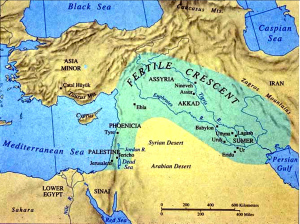
\includegraphics[scale=0.7]{sumermap}
\end{minipage}

\footnotetext{`Between two rivers,' namely the Tigris and Euphrates. As indicated on the map, these rivers formed the backbone of the \emph{Fertile Crescent,} in which early civilization, farming, crop and animal domestication occurred.}


\boldinline{Positional Enumeration}

The Babylonians used two symbols, roughly $\bone$ for 1 and $\bten$ for 10, likely made by the same stylus. Any number up to 59 was written with combinations, e.g.\par
\begin{minipage}[t]{0.8\linewidth}\vspace{-10pt}
	\[
		53=
		\begin{array}{c}
			\bten\!\bten\!\bten\\[-5pt]
			\bten\!\bten
		\end{array}
		\hspace{-7pt}
		\bone\!\bone\!\bone
	\]
\end{minipage}
\hfill
\begin{minipage}[t]{0.19\linewidth}\vspace{0pt}
	\flushright
	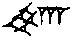
\includegraphics{babylon53}
\end{minipage}
\medbreak
with the picture showing a typical appearance as cuneiform. Arguably the greatest mathematical advance of the Babylonians was in evidence by 2000\BC{}; a \emph{positional} number system. To understand what this means, consider our decimal (base-10) system where 3835 uses the same symbol 3 to represent two different concepts 3000 and 30. We might write this as
\[
	3835=3\cdot 10^3+8\cdot 10^2+3\cdot 10+5
\]
Babylonian enumeration did exactly the same thing base-60; we call it a \emph{sexagesimal} system. The sexagesimal decomposition of 3835 is
\[
	3835=1\cdot 60^2+3\cdot 60+55
\]
for which the Babylonians would write
\[
	\vee\quad \vee\!\vee\!\vee\quad 
	\begin{array}{c}
		\bten\!\bten\!\bten\\[-5pt]
		\bten\!\bten
	\end{array}
	\hspace{-8pt}
	\begin{array}{c}
		\bone\!\bone\!\bone\\[-5pt]
		\bone\!\bone
	\end{array}
	\tag{$\ast$}
\]
In a positional system the meaning of a symbol depends on its position. For us, `3' might mean 30, 3000 or $\frac 3{1000}$, while for the Babylonians $\vee$ could mean 1, 60, 3600, 216000, or fractions such as $\frac 1{60},\frac 1{3600}$, etc. There was no symbol for zero (as a placeholder) until very late in Babylonian history, nor any \emph{sexagesimal point,} so determining position on ancient tablets can be difficult. For instance, ($\ast$) might instead have represented
\[
	60+3+\tfrac{55}{60}=63\tfrac{11}{12}\quad\text{or}\quad 60^3+3\cdot 60^2+55\cdot 60=230100
\]
To make things easier to read, we will write a sexagesimal number using commas to separate terms and, if necessary, a semicolon to denote the sexagesimal point. Thus
\[
	23,12,0;15=23\cdot 60^2+12\cdot 60+\frac{15}{60}=83520\frac 14
\] 

\boldinline{Why base 60?}

There are many theories, but no-one is sure precisely why. Here are some ideas.
\begin{itemize}
  \item 60 has many proper divisors (1, 2, 3, 4, 5, 6, 10, 12, 15, 20, 30). Many more numbers `divide exactly' than with decimal arithmetic: e.g., as a terminating sexagesimal, $\frac 13=\,;20$ is much simpler than the decimal $0.33333\ldots$
  \item A year has approximately 360 days (divisible by 60). The Babylonians were prolific astronomers and astrologers. Our modern usage of \emph{degrees, minutes, seconds} for angle, \emph{hours, minutes, seconds} for time, and the standard zodiac are all of Babylonian origin.
  \item The Babylonians possibly inherited two systems of counting (say base 10 and base 12) from older cultures and eventually combined them.
\end{itemize}
This is the sort of historical question that is rarely answerable in a satisfying way, particularly when discussing an ancient culture. Likely no-one `decided' to use base 60; like most culture, it probably happened slowly and organically, without much fanfare.
\smallbreak
It wasn't just counting that used 60s; units of Babylonian measure often used 60 when moving up and down the magnitude scale similarly to how we use multiples of 1000 (e.g.{} joules $\rightarrow$ kilojoules $\rightarrow$ megajoules). 


\boldinline{Calculations}\phantomsection\label{babmult}

Addition and subtraction of sexagesimals would have been as natural to the Babylonians as decimal calculations are to us. For instance, we might write
\[
	\begin{array}{rr@{,}r}
		&21&49\\
		+&3&37\\\hline
		+&2\overset{1}{4}&26\\
	\end{array} 
	\tag{i.e.{} $1309+217=1526$}
\]
Note how we carry 60s just like we are used to doing with 10s in decimal arithmetic: $49+37=1,26$.
\smallbreak

Multiplication is significantly harder. To mimic our decimal long-multiplication process would require knowing up to the 59 times table! For small products this might have been fine, but there is evidence that the Babylonians used two expressions to represent any product in terms of squares
\[
	xy=\frac 12\bigl[(x+y)^2-x^2-y^2\bigr]=\frac 14\bigl[(x+y)^2-(x-y)^2\bigr]
\]
Tablets consisting of tables of squares have been found, thus greatly aiding the computation of large products. For instance, to compute $31\times 22=682$,
\[
	31\times 22=\frac 14\bigl[53^2-9^2\bigr] =\frac 14\bigl[46,49-1,21\bigr] =\frac 14\bigl[45,28\bigr] =11,7+15=11,22
\]
This process would be combined with long-multiplication to multiply larger numbers.
% \[\begin{array}{rr@{}r@{;}}
% &&49\\
% \times&&37\\\hline
% &5,&43\\
% +&24,&30\\\hline
% &30,&13
% \end{array}\]
% Our first calculation reads $49\times 7=343=5,43$. The second reads $49\times 30=24\cdot 60+30$. These are then summed to obtain $49\cdot 37=1813=30\cdot 60+13$.


\boldinline{Fractions/Division}\phantomsection\label{babfraction}

The Babylonians used sexagesimals rather than fractions. They produced tables of reciprocals $\frac 1n$ which could be used to quickly evaluate divisions via $m\div n=m\times \frac 1n$. For instance
\[
	\frac 1{18}=0;3,20 \implies \frac{23}{18}=23(0;3,20) =1;9+0;7,40 =1;16,40
\]
This works nicely provided the only primes dividing $n$ are 2, 3 and 5, since any such $\frac 1n$ will be an exact terminating sexagesimal.\footnote{This is analogous to the fact that $\frac 1n$ has a terminating decimal if and only if the only primes dividing $n$ are 2 and 5.}
\smallbreak
For reciprocals without terminating sexagesimals, approximations were used; a scribe would simply choose a nearby denominator with a exact sexagesimal and state that the answer was approximate
\[
	\frac{11}{29}\approx\frac{11}{30}=11(0;2)=0;22
\]
More accuracy could be obtained by choosing a larger denominator. For instance, if a scribe wanted to divide by 11, they might observe that $11\cdot 13=143\approx 144$ and write\footnote{In fact, being rational, $\frac 1{11}=0.09090909\ldots=0;5,27,16,21,49,5,27,16,21,49,\ldots$ has a repeating sexagesimal expansion. This can be found by iteration, though it is time-consuming:
\[
	\frac{60}{11}=5\frac 5{11},\quad \frac{5\cdot 60}{11}=27\frac 3{11},\quad \frac{60\cdot 3}{11}=16\frac{4}{11},\ldots
\]
}
\[
	\frac 1{144}=0;0,25\implies \frac 1{11}\approx\frac{13}{144}=0;5,25
\]
which is 99.3\%{} accurate. Scribes were explicit in acknowledging that, say, ``11 does not divide,'' and that the result is an approximation. Remember that a single digit in the second sexagesimal place means only $\frac 1{3600}$, so even the most demanding application doesn't require many terms! The denominators in some of these tables were enormous, so far greater accuracy was often possible.
\medbreak


Another table listed all the ways an integer $<10$ could be multiplied exactly to get 10.
\[
	\begin{array}{@{}cl@{\qquad\qquad}cl}
		1&10&5&2\\
		2&5&6&1\ 40\\
		3&3\ 20&8&1\ 15\\
		4&2\ 30&9&1\ 6\ 40
\end{array}
\]
We omit the commas for separation and the sexagesimal point, as they did not exist.  Note also that 7 is missing since $\frac 17$ (and thus $\frac{10}7$) is not an exact sexagesimal. It should be clear from the table that
\[
	\frac{10}6=1;40\quad\text{and}\quad \frac{600}9=1,6;40
\]
In the latter case, note that $600=10\cdot 60$ would be written the same as 10, so this amounts to moving the sexagesimal point in $\frac{10}9=1;6,40$.

\vfil\goodbreak


\boldinline{Linear Systems}

These were solved by a mixture of the false position method (guess and modify as done by the Egyptians) and an approach modelled on homogeneous equations. For instance, here is a Babylonian approach to solving the following system
\[
	\begin{cases}
		3x+2y=11\\
		2x+y=7
	\end{cases}
\]
\begin{enumerate}
  \item Choose an equation, say the second, and set $\hat x=\hat y$. Now solve, for instance using false position to obtain $\hat x=\frac 73=2;20$.
  \item All solutions to the second equation have the form $x=\hat x+d$ and $y=\hat y-2d$, since $(d,-2d)$ is the general solution to the homogeneous equation $2x+y=0$. Substitute into the first equation:
  \[
  	11=3\left(\frac 73+d\right)+2\left(\frac 73-2d\right)=11+\frac 23-d\implies d=\frac 23
  \]
  \item Now solve $x=\frac 73+\frac 23=3$, $y=\frac 73-\frac 43=1$.
\end{enumerate}\smallskip

Step 2 should should remind you of the `nullspace' method from modern linear algebra: all solutions to the matrix equation $(2\ 1)\stwovec xy=7$ have the form
\[
	\twovec xy=\twovec{x_0}{y_0}+\vn
\]
where $\stwovec{x_0}{y_0}$ is some particular solution (here $x_0=y_0=\frac 73$) and $\vn=\stwovec d{-2d}$ lies in the nullspace of the (row) matrix $(2\ 1)$.


\boldinline{The Yale Tablet (YBC 7289)}\phantomsection\label{ybc7289}

One of the most famous tablets concerns an approximation to $\sqrt 2$. YBC stands for the \emph{Yale Babylonian Collection} which contains over 45,000 objects. The tablet is shown below along with an enhanced representation of the numerals.
\begin{center}
	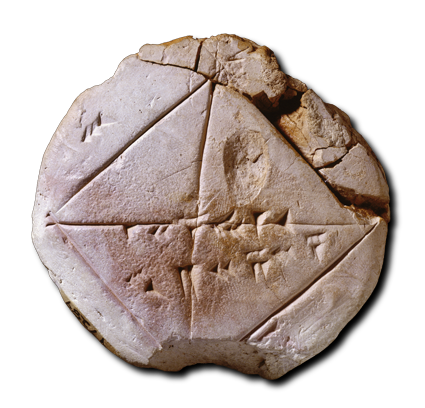
\includegraphics[height=160pt]{YBC7289.png}
	\qquad
	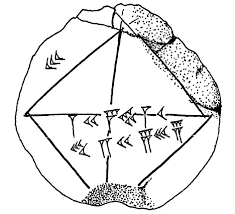
\includegraphics[height=140pt]{ybc.png}
\end{center}

The tablet depicts a square of side 30 (or possibly $\frac 12=0;30$) and labels the diagonal in two ways:
\begin{itemize}\itemsep0pt
  \item $1;24,51,10$ as an approximation to $\sqrt 2$, an underestimate by roughly 1 part in 2.5 million!
  \item $42;25,35$ as an approximation to the diagonal when the side is 30.
\end{itemize}
The Babylonians more often used the simpler approximation $1;25=1.41666\ldots$ which is still very close. Given the impractical accuracy of this approximation, it is reasonable to ask how it was obtained. No-one knows for certain, but two methods are theorized since both were used to solve other problems. It should be stressed that no Babylonian \emph{proofs} of these approaches are known.

\begin{description}\phantomsection\label{babroot}
	\item[1:\lstsp Square root approximation] $\sqrt{a^2\pm b}\approx a\pm\frac b{2a}$. This is essentially the linear approximation from elementary calculus. The idea is to choose a rational number for $a$ whose square is very close to 2, then the error should be very small. For instance:
	\begin{itemize}
  	\item $\sqrt 2=\sqrt{1+1}\approx 1+\frac 12=1;30$
  	\item $\sqrt 2=\sqrt{\left(\frac 43\right)^2+\frac 29}\approx\frac 43+\frac{2/9}{8/3}=\frac 43+\frac 1{12}=\frac{17}{12}=1;25$
  	\item $\sqrt 2=\sqrt{\left(\frac 75\right)^2+\frac 1{25}}\approx \frac 75+\frac{1/25}{14/5}=\frac{99}{70}=1;24,51,25,42,51,25,42,51,\ldots$
	\end{itemize}
	
	\item[2: Method of the Mean]\phantomsection\label{methodmean} It is easily checked (Exercise \ref{exs:methodmean}) that any sequence defined by the recurrence relation $a_{n+1}=\frac{a_n+2/a_n}2$ converges to $\sqrt 2$. Let us apply this to the sequence starting with $a_n=1$.
	\begin{gather*}
		a_1=1,\quad a_2=\frac 32=1;30,\quad a_3=\frac{17}{12}=1;25\\
		a_4=\frac{577}{408}=1+\frac{169}{408}=1;24,51,10,35,17,\ldots\\
		a_5=\frac{665857}{470832}=1;24,51,10,7,46\ldots
	\end{gather*}
	It seems incredible that any ancient culture would have bothered to go so far with these calculations to obtain the observed accuracy.\smallbreak

	The same analysis can be used to approximate other roots. For example, we could start with with $a_1=3$ to approximate $\sqrt{11}$ via $a_{n+1}=\frac 12(a_n+\frac{11}{a_n})$:
	\[
		a_2=\frac{10}3=3;20,\quad a_3=\frac{199}{60}=3;19,\quad a_4=\frac{79201}{23880}=3;18,59,50,57,17,\ldots
	\]
\end{description}




\boldinline{Quadratic Equations}

The above methods could be used to solve general quadratic equations. A question might be phrased as follows:
\begin{quote}
	I added twice the side to the square; the result is $2,51,40$. What is the side?
\end{quote}
In modern language, we want the solution to $x^2+2x=2\cdot 60^2+51\cdot 60+40=10300$.\smallbreak
Questions such as these were solved using templates. In the above example, the template is for solving $x(x+p)=q$ where $p,q>0$. Other templates were required for the other types of quadratic equation ($x^2=px+q$, etc.), since the Babylonians did not recognize negative numbers. Here is their algorithm applied to a simpler equation $x^2+4x=2$:\smallbreak
Set $y=x+p$ \ ($y=x+4$) then the equation can be decoupled:
\begin{align*}
	&
	\begin{cases}
		xy=q\\
		y-x=p
	\end{cases}
	&&
	\begin{cases}
		xy=2\\
		y-x=4
	\end{cases}
\end{align*}
Use this to solve for $x+y$:
\begin{align*}
	4xy+(y-x)^2&=p^2+4q &4xy+(y-x)^2&=4^2+4\cdot 2\\
	(y+x)^2&=p^2+4q &(y+x)^2&=24\\
	x+y&=\sqrt{p^2+4q} &x+y&=\sqrt{24}\approx\,4;54
\end{align*}
where the square-root was approximated using one of the earlier algorithms, e.g.
\[
	\sqrt{24}=\sqrt{5^2-1}\approx 5-\frac{1}{10}=4;54
\]
Since $x+y$ and $x-y$ are now known, false position could then be used to find
\[
	x=\frac{\sqrt{p^2+4q}-p}2 \hspace{50pt} x\approx 0;27
\]
You should recognize the method of completing the square and the quadratic formula; this approach is at least 4000 years old!
\smallbreak
While we've written this abstractly, in practice Babylonian scribes/students would be copying from a particular example of the same type. There were no abstract formulæ and everything was done without the benefit of any of our modern notation. We moreover have no written explanation from the Babylonians of what they were doing; typically all historians have to work with is the right-hand column of numbers and several examples like it!
\smallbreak
Note that the template only found the positive solution; the Babylonians had no notion of negative numbers. Amazingly, the Babylonians were also able to address certain cubic equations similarly.

\vfil\goodbreak



\boldinline{Pythagorean Triples}

Among the many tables of values created by the Babylonians are lists of Pythagorean triples. The Plimpton 322 tablet (also at Yale) has a large number of these (albeit with some mistakes).
\begin{center}
	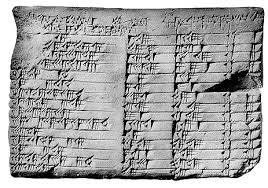
\includegraphics{plimpton322.jpg}
\end{center}
Due to the strange way in which the triples were encoded, it took a long time for scholars realized what they had. The table is also broken on the left so some columns are probably missing. %The triples are encoded as rational solutions to the equation $v^2=1+u^2$ rather than explicitly as integers.
\goodbreak

As an example, line 15 of the table describes the Pythagorean triple $53^2=45^2+28^2$ as follows.
\begin{itemize}
  \item The first entry is $(\frac{53}{45})^2=1;23,13,46,40$ (exact).
  \item The second entry is 28.
  \item The third entry is 53.
  \item The last two entries indicate line number 15.
\end{itemize}
The first three (interesting) entries are therefore $((\frac ca)^2,b,c)$ where $c^2=a^2+b^2$. It is possible that a missing column of the tablet explicitly mentioned $a$.
\smallbreak 

It is not known how the table was completed, although the first column exhibits a descending pattern that provides clues to its construction. One theory is that a scribe found rational solutions to the equation $v^2=1+u^2$ (equivalently $(v+u)(v-u)=1$) by starting with a choice of $v+u$ and using a table of reciprocals to calculate $v-u$.
\smallbreak
To revisit our example, if $v+u=\frac 95=1;48$, then
\[
	v-u=\frac 1{v+u}=\frac 59=0;33,20
\]
and we have a linear system of equations for $u,v$ whose solutions are
\[
	v=1;10,40=\frac{53}{45},\quad u=0;37,20=\frac{28}{45}
\]
We investigate this further in Exercise \ref{exs:plimpton}. The Plimpton tablet has been the source of enormous scholarship; look it up!


\boldinline{Geometry}

The Babylonians also discusses many geometric problems. They used both $\pi\approx 3$ and $\pi\approx 3\frac 18$ to approximate areas of circles. They had calculations (both correct and erroneous) for the volume of a frustrum (truncated pyramid). They also knew that the altitude of an isosceles triangle bisects its base and that the angle in semicircle is a right angle. None of these statements were presented as theorems in a modern sense; we merely have computations that use these facts. We simply don't know how deep the Babylonian understanding of these principles was.

\boldsubsubsection{Summary}

\begin{itemize}
  \item Sexagesimal positional enumeration. No zero or fractions. 
  \item More advanced than Egyptian mathematics but still practical/non-abstract. Perhaps only appears more advanced because we have much more evidence (1000s of tablets versus a handful of papyri). Like Egypt, we have worked examples without abstraction or any statement of general principles.
  \item Some distinction (`does not divide') between approximate and exact results.
  \item Limited geometry compared to algorithmic/numerical methods.
\end{itemize}

\vfil\vfil\goodbreak


\begin{exercises*}{}{}
	There is no single `correct' way to do Babylonian calculations. The goal is simply to play with the ideas; use enough notation to get a feel for it without torturing yourself.
	
	\begin{enumerate}%\setcounter{enumi}{1}
	  \item %[1-18]
	  Convert the sexagesimal values $0;22,30$, \ $0;8,6$, \ $0;4,10$ and $0;5,33,20$ into ordinary fractions in lowest terms.
	  
	  
	  \item\begin{enumerate}%[1-20]
	    \item \makebox[220pt][l]{Multiply 25 by $1,4$\hfill(b)}\lstsp Multiply 18 by $1,21$.
	    \item[](\emph{Either compute directly (long multiplication) or use the difference of squares method on page \pageref{babmult}})
	  \end{enumerate}
	  
	  
	  \item\begin{enumerate}%[1-20]
	    \item \makebox[220pt][l]{Use reciprocals to divide 50 by 18.\hfill (b)}\lstsp Repeat for $1,21$ divided by 32.
	  \end{enumerate}
	  
	  
	%   \item[1-22] The approximation for area $A_\circ =\frac 1{12}C^2$ is equivalent to $\pi=3$. Draw a circle circumscribing an equilateral triangle. Suppose that $\frac 13$ of the circumference is $a$ and that the radius is $r$. The area of half the bulls-eye is then $\frac 13$ the area of the circle minus the area of the isosceles triangle with legs $r$ and angle $120^\circ$.\\
	%   In radians, we clearly have $a=\frac{2\pi r}3$. Using the Babylonian approximation for $\pi$, this yields $a=2r$. The isosceles triangle has the same area as an equilateral triangle of side length $r$: this is $\frac{\sqrt 3}4r^2$. Using the Babylonian $\sqrt 3\approx\frac 74$, and our expression for $r=\frac 12a$, we obtain $A_\triangle=\frac {7a^2}{16}$.\\
	%  $A_\circ=\frac 1{12}C^2$ with $C$ the circumference yields $A_\circ=\frac 34a^2$. Thus the area of the bulls-eye is
	% \[2\left(\frac 13A_\circ-A_\triangle\right)=2\left(\frac{a^2}4-\frac {7a^2}{64}\right)=\frac{9a^2}{32}\]
	% The long transversal of the bulls-eye is the chord of the circle made by an edge of the original equilateral triangle: this length is $\sqrt 3r\approx\frac 74\cdot\frac a2=\frac{7a}8$.\\
	% The short transversal is $r\approx \frac a2$.
	
	
		\item Use the Babylonian method of false position to solve the linear system $\begin{cases}
		3x+5y=19\\
		2x+3y=12
		\end{cases}$
	  
	  
	  \item%[1-24]
	  \begin{enumerate}
	    \item Convert the approximation $\sqrt 2\approx 1;24,51,10$ to a decimal and verify the accuracy of the approximation on page \pageref{ybc7289}.
	    \item Multiply by 30 to check that the length of the diagonal is as claimed.
	  \end{enumerate}
	  
	  
	  \item Babylonian notation is not required for this question.
	  \begin{enumerate}
	    \item Use the square root approximation (pg.\,\pageref{babroot}) with $a=\frac 83$ to find an approximation to $\sqrt 7$.
	    \item Taking $a_1=3$, apply the method of the mean to find the approximation $a_3$ to $\sqrt 7$.
	  \end{enumerate}
	  
	  
	  \item\label{exs:plimpton}%[1-26]
	  Recall that $v^2=1+u^2$ in the construction of the Plimpton tablet.
	  \begin{enumerate}
	    \item If $v+u=\alpha$, show that $u=\frac 12(\alpha-\alpha^{-1})$ and $v=\frac 12(\alpha+\alpha^{-1})$.
	    \item Suppose $v+u=1;30=\frac 32$. Find $u,v$ and the corresponding Pythagorean triple.
	  	\item Repeat for $v+u=1;52,30=\frac{15}8$.
	  	\item Repeat for $v+u=2;05=\frac{25}{12}$. This is line 9 of the tablet.
	  	%\item Repeat for $v+u=\frac{20}9=2;13,20$.
	  \end{enumerate}
	
	  
	  \item%[1-32] 
	  Solve the following problem from tablet YBC 4652. I found a stone, but did not weigh it; after I subtracted one-seventh, added one-eleventh (of the difference), and then subtracted one-thirteenth (of the previous total), it weighed 1 \emph{mina} ($=60$ \emph{gin}). What was the stone's weight?\par
	  (\emph{Make your best guess as to the meaning of the problem, it might not be clear!})
	  
	  
	  \item%[1-34]
	  Solve the following problem from tablet YBC 6967. A number exceeds its reciprocal by 7. Find the number and the reciprocal.\par
	  (\emph{In this case, two numbers are reciprocals if their product is 60})
	
	
	  \item (Hard)\lstsp For this question it is helpful to think about the corresponding facts for decimals.
	  \begin{enumerate}
	    \item Explain the observation on page \pageref{babfraction} regarding which reciprocals $n$ have a terminating sexagesimal. Can you prove this?
	  	\item Find the periodic sexagesimal representation of $\frac 17$ and use geometric series \emph{prove} that you are correct.
	  \end{enumerate}  
	  
	  
	  \item\label{exs:methodmean}
	  For this question, look up the AM--GM inequality and remind yourself of some basic Analysis.
	  \begin{enumerate}
			\item Suppose $(a_n)$ is a sequence satisfying the recurrence $a_{n+1}=\frac 12(a_n+\frac 2{a_n})$. Prove that $a_n\ge \sqrt 2$ whenever $n\ge 2$.
			\item Prove that $a_n\to\sqrt 2$.
	% 		\[0\le a_{n+1}-\sqrt 2=\frac 12(a_n-\sqrt 2)+\frac{\sqrt 2-a_n}{\sqrt 2a_n}\le\frac 12(a_n-\sqrt 2)\]
	% 	so that $\lim\limits_{n\to\infty}a_n=\sqrt 2$.
		\end{enumerate}
	\end{enumerate}
\end{exercises*}

% 
% In other situations a two position approximation might be used, for instance
% \[\frac 1{11}=0.09090909\ldots=;5,27,16,21,49,5,27\ldots\]
% which could then be used to divide:
% \[25\div 11=25\cdot(;5,27,16,\ldots)=2;16,21,\ldots\]
% %(working: $25\cdot 16=400=6;40$, $25\cdot 27=675=11;15$, $25\cdot 5=125=2;5$).
% Similarly,
% \[\frac 17=0.142857142857\ldots=;8,34,17,8,34,17,\ldots\]
% yields
% \[10\div 7=10\cdot(;8,34,17,\ldots)=1;25,42,\ldots\]